\documentclass{article}
\usepackage{hyperref}
\usepackage{verbatim}
\usepackage{graphicx}
\usepackage{xcolor}
\usepackage{tikz}
\usepackage{lscape}
\usepackage{pgfgantt}
\usepackage{cleveref}
\usepackage[a4paper,margin=1in]{geometry}
\usepackage{calc}
\usepackage{enumitem}
\usetikzlibrary{patterns}
\usetikzlibrary{calc}
\usetikzlibrary{decorations.pathmorphing}
\usetikzlibrary{shapes}
% \usepackage{url}
\graphicspath{{./images/}}
\usepackage{wrapfig}
\usepackage[numbers]{natbib}
\newcommand{\itm}[1]{\begin{itemize} #1 \end{itemize}}
\newcommand{\num}[1]{\begin{enumerate} #1 \end{enumerate}}
\newcommand{\desc}[1]{\begin{description} #1 \end{description}}
%\newcommand{\descalign}{[leftmargin=!,labelwidth=\widthof{\bfseries #1}]}
\newcommand{\sctn}[1]{\section{#1} }
\newcommand{\ssctn}[1]{\subsection{#1} }
\newcommand{\sssctn}[1]{\subsubsection{#1} }
\newcommand{\img}[2]{\includegraphics[scale=#1]{#2}}
\newcommand{\rarr}{$\rightarrow$ }
\newcommand{\bld}[1]{\textbf{#1}}
\newcommand{\itl}[1]{\textit{#1}}
\newcommand{\ctr}[1]{\begin{center} #1 \end{center}}
\newcommand{\fig}[3]{\ctr{\begin{figure}[htbp] #1 \caption{#2} \label{fig: #3} \end{figure}}}
\newcommand{\wrp}[1]{\begin{wrapfigure}{r}{0.25\textwidth}
						\centering
							#1
					 \end{wrapfigure}}

\newcommand\ytl[2]{
\parbox[b]{8em}{\hfill{\color{black}\bfseries\sffamily #1}~$\cdots\cdots$~}\makebox[0pt][c]
{$\bullet$}\vrule\quad \parbox[c]{12.5cm}
{\vspace{8pt}\color{black!40!black!80}\raggedright\sffamily #2.\\[15pt]}\\[-3pt]}
\newcommand{\kmd}{KoMoDo}

\title{KoMoDo++: An enhanced assembler-level development environment for the 32-bit ARM chip}
\author{Houman Brinjcargorabi\\Supervised by Prof. David Brailsford\\\\
\includegraphics[scale=0.4]{UoN_arms}}%
%
%
\begin{document}
\pagenumbering{gobble}
\thispagestyle{empty}

\maketitle{}
\begin{abstract}
\noindent KoMoDo is an existing development environment for the assembly-level programming of the 32-bit ARM chip. It was originally developed at the University of Manchester where it is used at both the Undergraduate and Masters level. KoMoDo allows for development either at the PC-board level for actual ARM-chip programming or, alternatively, it can offer an emulated environment for the ARM chip using a simulated set-up known as the `jimulator'. It is this latter environment that is in use at Nottingham.\\\\
%
Whether downloading developed code to an actual ARM chip, or to the jimulator, these two possible options share a common top-level screen display (showing memory, register contents etc.) which is KoMoDo itself.\\\\
%
The aim of this project is to modernize and improve upon the KoMoDo interactive environment by enhancing the display of such features as single stepping, register contents and memory contents. Facilities of this sort enable students to learn about the intricacies of the machines and languages they work with.\\\\
%
Over time KoMoDo has become dated and component packages that were once in their prime are now outdated and hard to find. A thorough upgrade is needed even for the basic components of the system. The desired outcome of this project is to create KoMoDo++ using modern software frameworks, while still relying on the jimulator as the ARM emulator.

% A critical application used by many students in their studies in nottingham aswell as in manchester
% Used to teach students the very basics of a computers architecture aswell as introducing them to machine code
% Needs to be updated so that students can still use it, at nottingham it's one of the only ways students can try a linux flavour

\end{abstract}
\pagebreak
\tableofcontents
\pagebreak
\pagenumbering{arabic}
%\let\clearpage\relax
% !TEX root = ./main.tex
\sctn{Background}
KoMoDo is an interactive screen-display tool, using X-Windows on the Unix/GNU Linux architecture. It was originally designed by Charlie Brej of the Dept. of Computer Science, University of Manchester. The majority of the current maintenance is handled by Jim Garside -- a senior lecturer at the University of Manchester.\\\\
%
The early history of KoMoDo is hazy but it was built using GLib and GTK 1.2 which both date back to 1999.\\\\
%
KoModo is used to teach students the low-level architecture of modern computers. The University of Nottingham uses it as a tool in the first year for the core module G51CSF. It provides an environment in which students can learn about machine code and learn the complexities of instruction design.\\\\
%
KoMoDo teaches students to think about the programs they write in a low-level manner, which is close to the `bare metal'. This is in contrast to the more abstract style of a typical high-level language.\\\\
%
KoMoDo, in the context of a teaching aid, is primarily run in emulation mode. The back-end emulator running as a process, accessed via a two-way Unix pipe, is called the jimulator. The jimulator is the driving force behind KoMoDo.\\\\
%
KoMoDo also uses a disassembler called chump (if rendered upside down in an unknown font it spells `dump'). Chump is used to convert the resulting assembler instructions back to something that KoMoDo can use and display to the user.\\\\
%
Appreciation for KoMoDo runs deep. Although first year students do not generally realise the importance of KoMoDo until much later on in their degree course, it is nevertheless  important to keep it alive and fully functional.
%
\sctn{Aims and Objectives}
\ssctn{Aims}
The aim of this project is to redesign KoMoDo and provide it with much needed enhancements and features. The enhancements will come in several forms; a revamped user interface, a better user experience and syntax-highlighted ARM instructions. KoMoDo's portability to platforms other than Linux is also on the agenda. For the duration of this project Linux will remain the primary target platform. Students receive exposure to Linux only via the use of KoMoDo so it is a primary goal to ensure full functionality in the Linux ecosystem.
\ssctn{Objectives}
\itm{
	\item Dissect KoMoDo \itm{
			\item Discover how KoMoDo communicates with the jimulator
			\item Discover how memory is shared between the jimulator and KoMoDo
			\item Discover how Chump is used to show disassembled ARM instructions
		}
	\item Future proof KoMoDo \itm{
			\item Use a well established framework such as QT
			\item Ensure libraries used are easily changed and or updated
			\item Develop a modern UI and improved UX
		}
	\item Portability and Platforms \itm{
			\item Ensure KoMoDo++ works on Linux distributions
			\item Make moves towards ensuring KoMoDo++'s use on multiple platforms
		}
	\item Stretch goals \itm{
			\item Convert the jimulator to work independently of the platform
			\item Convert Chump to work independently of the platform
			\item Convert the assembler to work independently of the platform
		}
}
%Portability of KoMoDo will be achieved using QT, a framework designed with cross compilation in mind. QT provides a meta-object compiler which enriches the C++ language providing cross compilation support. QTs enrichments also mean that the model-view-controller pattern is further simplified. QTs solution to messaging between views is to allow users to subscribe to events. Furthermore said events contact the subscriber when an event is triggered.
% modernize komodo by
	% changing the UI
	% Improving the UX
	% Adding new features
		% syntax highlighting
	% future proofing with regards to portability

%Ensure it works on linux becase currently thats the only exposure students recieve within the university
% primary objectives
	% Ensure it runs on linux
	% Disect KoMoDo
		% Find out how KoMoDo uses the jimulator
		% Work on how the memeory should be presented

% Stretch Goals
	% Modify AASM to work on any platform
	% Modify the jimulator to work on any platform

\sctn{External Interests}
The University of Manchester where KoMoDo was originally conceived still uses KoMoDo as a teaching aid. Several other universities including the University of Nottingham are also still using it to teach students the fundamentals of computer architecture. It is in the interest of the aforementioned universities that KoMoDo is able to be used by students regardless of platform and library dependencies.
% Working with Manchester University to improve this learning tool
% A key tool used in teaching students about the inner workings of modern computers
	% ALlows students to experiment with the theory they learn
	% Changes the ways students percieve their applications, allows them to think more atomically
	% the atomic thinking is the bases of many courses such as concurrency and optimization

\sctn {Work Plan}
To fully realise the challenges of this project it is best to explore the main components for a UI/UX overhaul. First, it is important to understand how KoMoDo operates currently, how its UI was built and to identify any dependencies on other software. Secondly, we need to understand what frameworks are available and the feasibility of their use. \\\\
%
Once the research has been complete, via use cases, a system requirements specification can be derived to fully encapsulate KoMoDo++'s desired functionality. Moreover, this project will be carried out using the Agile methodology. Working using Agile means that the project aims will change to meet the desired outcomes.\\\\
%
A breakdown of the proposed time line is provided via a Gantt chart. Refer to figure \ref{fig: gantt} in the Appendix.

\sctn{KoMoDo}
KoMoDo utilises additional components to provide capabilities which allow users to emulate the 32-bit ARM chip. It communicates with the various components in different ways. For example communication between the Jimulator and KoMoDo occurs via a two-way Unix pipe in the form of commands defined by the Jimulator. This section aims to explore the communication between these various components and how they are integrated into KoMoDo. 

\ssctn{Chump}

\ssctn{Jimulator}

\include{qtresearch}
% !TEX root = ./main.tex
\graphicspath{ {images/requirements/} }

\sctn{Requirements}
This section is dedicated to capturing the requirements of potential users within the scope of KoMoDo's educational use. Personas will be created to conceptualise the requirements required to achieve the desired results. Personas or Characters are used to identify key stakeholders for an application. Developing personas provides insight into the applications usage and the desired behaviours expected by stakeholders.\\\\
%
System requirements should be malleable, transforming over time as use cases and users change. Change in the requirements over time allows the end product to better suit the software needs. Using the Agile development methodology allows for a reactive planning and development process, focusing on early delivery and continuous development \cite{wikipedia_agile_dev}.\\\\
%
The functional requirements of KoMoDo++ will be derived from the persona use cases.

\ssctn{Use Case}
To fully realise the required features of KoMoDo++, two separate personas have been created. The requirements specification will be created based on the use case for each persona. Use cases provide useful insight into the requirements of a particular type of user, based on their interactions with the system. Developing use cases helps model the context of the system as well as providing in-depth analysis into a user's needs, thereby aiding in creating a more refined set of requirements.\\\\
%
Personas are a tool to capture the context of use. Therefore, contrasting personas have been created to better reflect interactions with KoMoDo++. Moreover, personas provide insight which can help make informed architectural design decisions.
%
\sssctn{Personas}
\bld{Mike}\\
Mike is a first year computer scientist and one of his first set of modules involves learning about low-level hardware/software. Mike has made his own website before and did so using a text editor, he thought syntax highlighting made it easier for him to read the code. Mike has a particular interest in UI/UX design. Mike is a Windows user and has not used Linux before, but he thinks he will eventually use Linux. Mike sees that KoMoDo++ is one of the tools used to work on the coursework and so chooses to download it.\\\\
%
\bld{Lucy}\\
Lucy is a third year computer scientist working on her dissertation. She has decided to create her own low-level language along with its own compiler. In her first year she learnt about the 32bit ARM chip architecture but she's forgotten some of the intricacies. She has decided she needs to brush up on the ARM-chip details and would find it useful if she could see a breakdown of changes that occur at each step. Lucy also uses a Macintosh as her daily computer. She downloads KoMoDo++ for the advanced features it provides.
%
\sssctn{Scenarios}
\bld{Scenario 1: Mike}\\
Mike has just been given his first assignment which asks him to implement a simple multiplication function using ARM32. He writes some of the code and runs KoMoDo++ for the first time on his Windows laptop. Mike takes note that the basic version of KoMoDo++ is simple and inviting to use. Consequently, he finds it is intuitive to get started and so immediately loads up his code. Mike starts stepping through the code to see how it transforms over time. He likes it that the ARM instructions in the memory window use syntax highlighting. He also likes the break down of what an instruction does.  Mike carries on slowly implementing his solution and finds KoMoDo++ easy to use.\\\\
%
\bld{Scenario 2: Lucy}\\
Lucy begins to design her machine language, she uses a simple program written in ARM32 as the basis for her design. She has not used KoMoDo++ yet and she notes that upon opening KoMoDo++ it was good that there was a breakdown of its features. She starts by stepping through the code in the advanced view and takes note about the flags that change. She is particularly pleased with the code breakdown because it gives her an insight into what the command does on-the-fly. Lucy carries on slowly building up her new language, referring to the decisions made for ARM32.

\ssctn{Use Case Diagrams}
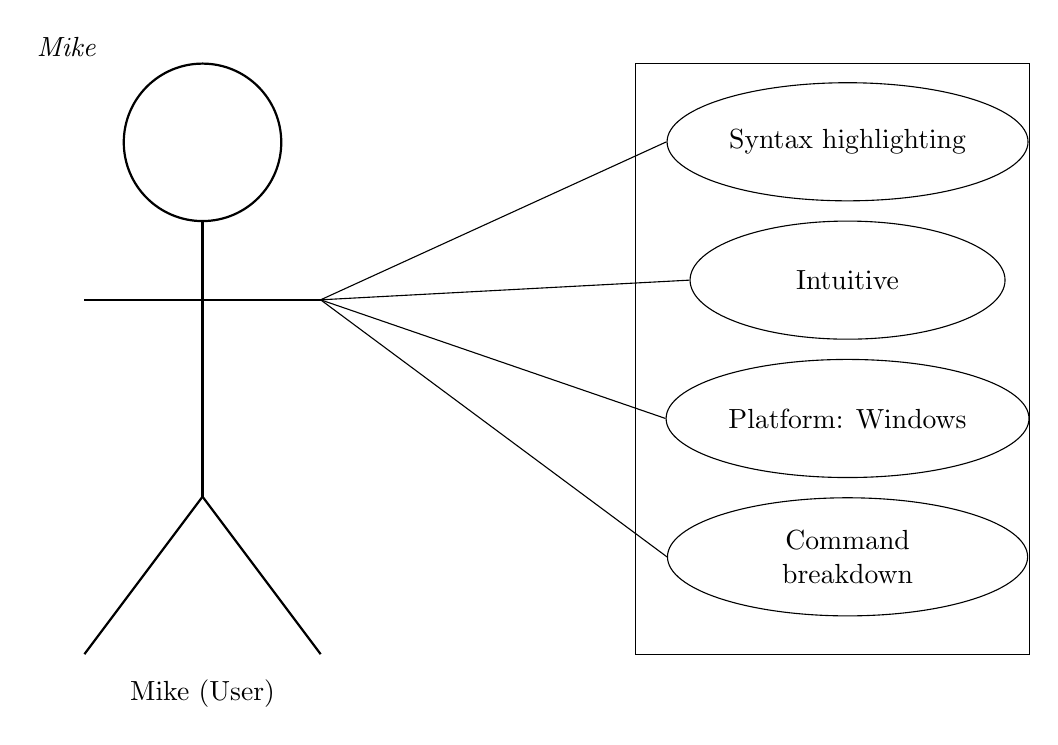
\begin{tikzpicture}[>=latex]
			%elements
			% \draw (0,0) circle (1cm);
			\node [thick] at (0,0) (head) [circle,draw, minimum width=20mm] {};
			\node at ($(head.north west) + (-1cm,0.5cm)$)[] {\itl{Mike}};
			%torso
			\draw [thick] (canvas cs:x=0cm,y=-10mm) -- (canvas cs:x=0cm,y=-4.5cm);
			%arms
			\draw [thick] (canvas cs:x=-1.5cm,y=-2cm) -- (canvas cs:x=1.5cm,y=-2cm);
			%right leg
			\draw [thick] (canvas cs:x=0cm,y=-4.5cm) -- (canvas cs:x=1.5cm,y=-6.5cm);
			%right leg
			\draw [thick] (canvas cs:x=0cm,y=-4.5cm) -- (canvas cs:x=-1.5cm,y=-6.5cm);
			%name
			\node at (canvas cs:x=0cm,y=-7cm) [] {Mike (User)};
			%requirements box
			\node at (canvas cs:x=8cm,y=-2.75cm) (box) [rectangle, draw=black!100, minimum width=5cm, minimum height=7.5cm] {};

			% requirements
			\node [right] at ($(box.north west) + (0.4cm, -1cm)$) (req1) [ellipse,draw=black!100,minimum width=4cm,minimum height=1.5cm] {Syntax highlighting};
			\node [] at ($(req1.south) + (0cm, -1cm)$) (req2) [ellipse,draw=black!100,minimum width=4cm,minimum height=1.5cm] {Intuitive};
			\node [] at ($(req2.south) + (0cm, -1cm)$) (req3) [ellipse,draw=black!100,minimum width=4cm,minimum height=1.5cm] {Platform: Windows};
			\node [] at ($(req3.south) + (0cm, -1cm)$) (req4) [ellipse,draw=black!100,minimum width=4cm,minimum height=1.5cm ,text width=3cm, align=center] {Command breakdown};


			\draw [] (req1.west) -- (canvas cs:x=1.5cm,y=-2cm);
			\draw [] (req2.west) -- (canvas cs:x=1.5cm,y=-2cm);
			\draw [] (req3.west) -- (canvas cs:x=1.5cm,y=-2cm);
			\draw [] (req4.west) -- (canvas cs:x=1.5cm,y=-2cm);
		\end{tikzpicture}
		\\\\\\
		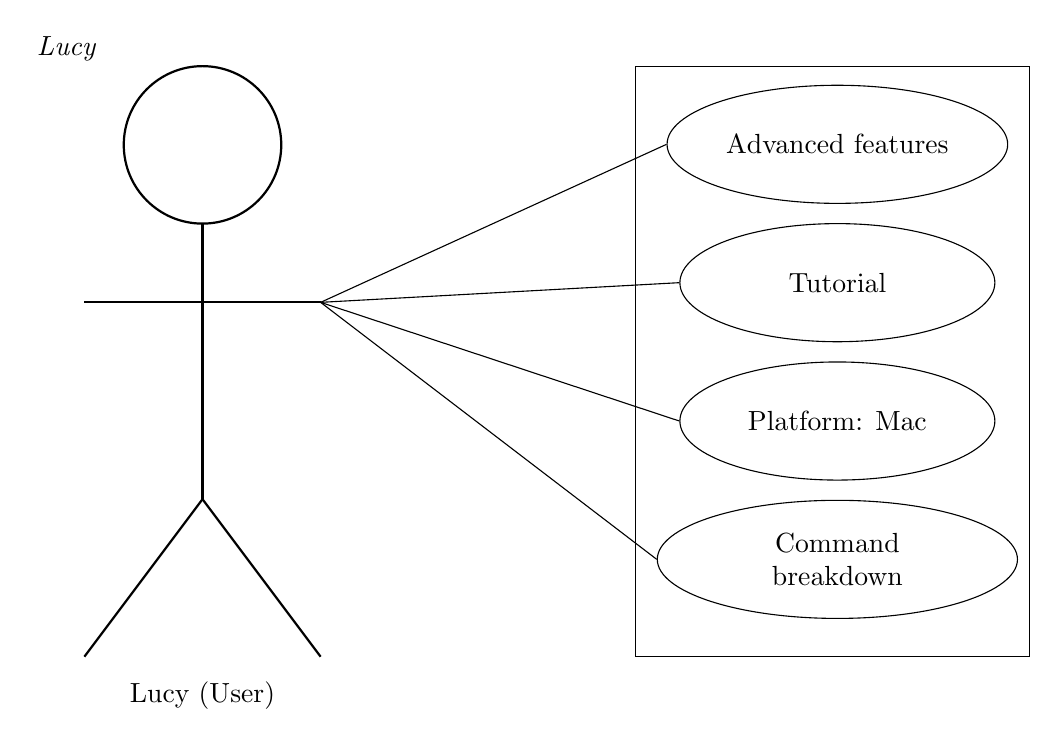
\begin{tikzpicture}[>=latex]
			%elements
			% \draw (0,0) circle (1cm);
			\node [thick] at (0,0) (head) [circle,draw, minimum width=20mm] {};
			\node at ($(head.north west) + (-1cm,0.5cm)$)[] {\itl{Lucy}};
			%torso
			\draw [thick] (canvas cs:x=0cm,y=-10mm) -- (canvas cs:x=0cm,y=-4.5cm);
			%arms
			\draw [thick] (canvas cs:x=-1.5cm,y=-2cm) -- (canvas cs:x=1.5cm,y=-2cm);
			%right leg
			\draw [thick] (canvas cs:x=0cm,y=-4.5cm) -- (canvas cs:x=1.5cm,y=-6.5cm);
			%right leg
			\draw [thick] (canvas cs:x=0cm,y=-4.5cm) -- (canvas cs:x=-1.5cm,y=-6.5cm);
			%name
			\node at (canvas cs:x=0cm,y=-7cm) [] {Lucy (User)};
			%requirements box
			\node at (canvas cs:x=8cm,y=-2.75cm) (box) [rectangle, draw=black!100, minimum width=5cm, minimum height=7.5cm] {};

			% requirements
			\node [right] at ($(box.north west) + (0.4cm, -1cm)$) (req1) [ellipse,draw=black!100,minimum width=4cm,minimum height=1.5cm] {Advanced features};
			\node [] at ($(req1.south) + (0cm, -1cm)$) (req2) [ellipse,draw=black!100,minimum width=4cm,minimum height=1.5cm] {Tutorial};
			\node [] at ($(req2.south) + (0cm, -1cm)$) (req3) [ellipse,draw=black!100,minimum width=4cm,minimum height=1.5cm] {Platform: Mac};
			\node [] at ($(req3.south) + (0cm, -1cm)$) (req4) [ellipse,draw=black!100,minimum width=4cm,minimum height=1.5cm ,text width=3cm, align=center] {Command breakdown};


			\draw [] (req1.west) -- (canvas cs:x=1.5cm,y=-2cm);
			\draw [] (req2.west) -- (canvas cs:x=1.5cm,y=-2cm);
			\draw [] (req3.west) -- (canvas cs:x=1.5cm,y=-2cm);
			\draw [] (req4.west) -- (canvas cs:x=1.5cm,y=-2cm);
		\end{tikzpicture}
    %
    %
  \ssctn{Software Requirement Specification}
  Prototyping is a key component of the Agile methodology, to do so two individual requirement specifications will be developed, one for the prototype and one for the final product. It is important to develop prototypes since they can quickly reveal issues with implementation considerations.
  %
  \sssctn{Prototype}
  The requirements for the prototype form the basis on which the final product will be built.\\\\
  %
  \itl{Functional requirements}\\
  \itm{
    \item Provide the same functionality as the current KoMoDo \itm{
        \item Register banks
				\item Memory view
        \item Breakpoints
        \item Single stepping
        \item Multi stepping
        \item Loading kmd files
        \item Compiling source files
      }
    \item Introduce no additional dependencies\\\\
  }
  %
  \itl{Non-functional requirements}\\
  \itm{
    \item Intuitive design \itm{
        \item Basic view mode
				\item Themes
				\item Action icons
      }
    \item Compatibility: Linux
    \item Similar responsiveness as the current KoMoDo
		\item Create installer for supported platforms\\
  }
  \sssctn{Final Product}
	\itl{Functional requirements}\\
	\itm{
    \item Provide the same functionality as the current KoMoDo \itm{
        \item Register banks \itm{
					\item notify user of register changes
				}
        \item Memory view
        \item Breakpoints
        \item Single stepping
        \item Multi stepping
        \item Loading KMD files
        \item Compiling source files
      }
    \item Introduce no additional dependencies
		\item Syntax highlighting
		\item Breakpoints integrated into memory window
		\item Ability to hide empty memory
		\item More complete build process
		\item Active memory jump-to
		\item Preferences
		\item Themes via XML files
		\item Instruction breakdown\\\\
  }
  %
  \itl{Non-functional requirements}\\
  \itm{
    \item Intuitive design \itm{
        \item Basic view mode
				\item Themes
				\item Action icons
      }
    \item Compatibility: Linux, Windows, Mac
    \item Similar responsiveness as the current KoMoDo
		\item Create installer for supported platforms
  }

\appendix
%\include{researchEditors}
%\include{researchStructures}
%% !TEX root = ./main.tex
\graphicspath{ {images/requirements/} }

\sctn{Requirements}
This section is dedicated to capturing the requirements of potential users within the scope of KoMoDo's educational use. Personas will be created to conceptualise the requirements required to achieve the desired results. Personas or Characters are used to identify key stakeholders for an application. Developing personas provides insight into the applications usage and the desired behaviours expected by stakeholders.\\\\
%
System requirements should be malleable, transforming over time as use cases and users change. Change in the requirements over time allows the end product to better suit the software needs. Using the Agile development methodology allows for a reactive planning and development process, focusing on early delivery and continuous development \cite{wikipedia_agile_dev}.\\\\
%
The functional requirements of KoMoDo++ will be derived from the persona use cases.

\ssctn{Use Case}
To fully realise the required features of KoMoDo++, two separate personas have been created. The requirements specification will be created based on the use case for each persona. Use cases provide useful insight into the requirements of a particular type of user, based on their interactions with the system. Developing use cases helps model the context of the system as well as providing in-depth analysis into a user's needs, thereby aiding in creating a more refined set of requirements.\\\\
%
Personas are a tool to capture the context of use. Therefore, contrasting personas have been created to better reflect interactions with KoMoDo++. Moreover, personas provide insight which can help make informed architectural design decisions.
%
\sssctn{Personas}
\bld{Mike}\\
Mike is a first year computer scientist and one of his first set of modules involves learning about low-level hardware/software. Mike has made his own website before and did so using a text editor, he thought syntax highlighting made it easier for him to read the code. Mike has a particular interest in UI/UX design. Mike is a Windows user and has not used Linux before, but he thinks he will eventually use Linux. Mike sees that KoMoDo++ is one of the tools used to work on the coursework and so chooses to download it.\\\\
%
\bld{Lucy}\\
Lucy is a third year computer scientist working on her dissertation. She has decided to create her own low-level language along with its own compiler. In her first year she learnt about the 32bit ARM chip architecture but she's forgotten some of the intricacies. She has decided she needs to brush up on the ARM-chip details and would find it useful if she could see a breakdown of changes that occur at each step. Lucy also uses a Macintosh as her daily computer. She downloads KoMoDo++ for the advanced features it provides.
%
\sssctn{Scenarios}
\bld{Scenario 1: Mike}\\
Mike has just been given his first assignment which asks him to implement a simple multiplication function using ARM32. He writes some of the code and runs KoMoDo++ for the first time on his Windows laptop. Mike takes note that the basic version of KoMoDo++ is simple and inviting to use. Consequently, he finds it is intuitive to get started and so immediately loads up his code. Mike starts stepping through the code to see how it transforms over time. He likes it that the ARM instructions in the memory window use syntax highlighting. He also likes the break down of what an instruction does.  Mike carries on slowly implementing his solution and finds KoMoDo++ easy to use.\\\\
%
\bld{Scenario 2: Lucy}\\
Lucy begins to design her machine language, she uses a simple program written in ARM32 as the basis for her design. She has not used KoMoDo++ yet and she notes that upon opening KoMoDo++ it was good that there was a breakdown of its features. She starts by stepping through the code in the advanced view and takes note about the flags that change. She is particularly pleased with the code breakdown because it gives her an insight into what the command does on-the-fly. Lucy carries on slowly building up her new language, referring to the decisions made for ARM32.

\ssctn{Use Case Diagrams}
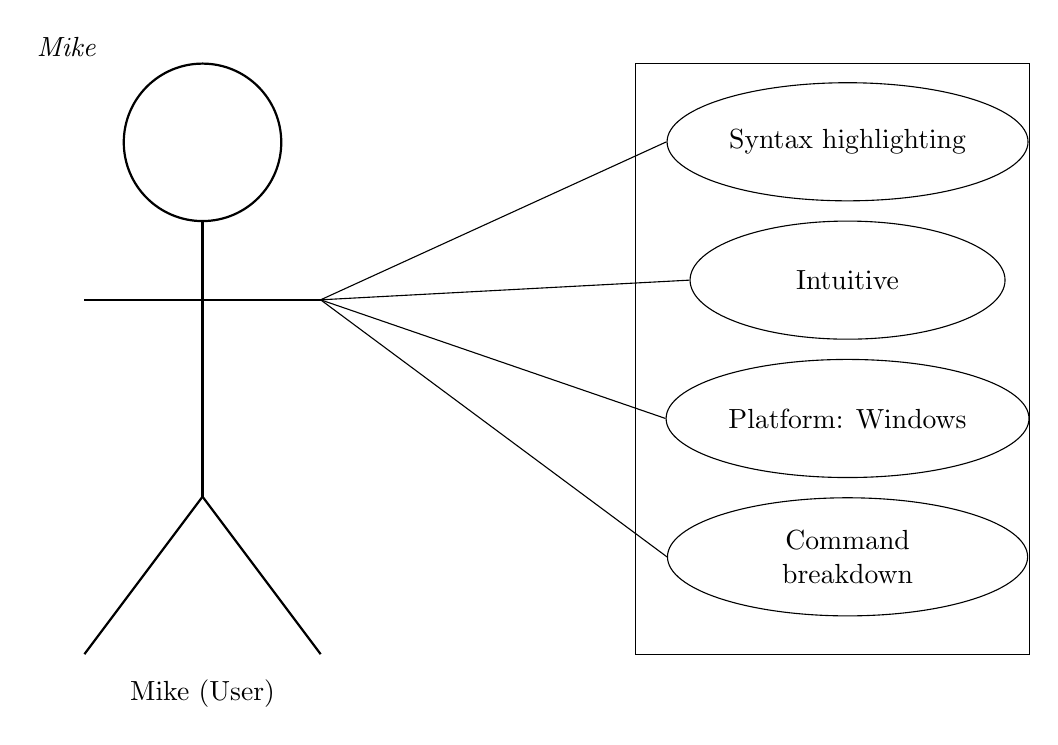
\begin{tikzpicture}[>=latex]
			%elements
			% \draw (0,0) circle (1cm);
			\node [thick] at (0,0) (head) [circle,draw, minimum width=20mm] {};
			\node at ($(head.north west) + (-1cm,0.5cm)$)[] {\itl{Mike}};
			%torso
			\draw [thick] (canvas cs:x=0cm,y=-10mm) -- (canvas cs:x=0cm,y=-4.5cm);
			%arms
			\draw [thick] (canvas cs:x=-1.5cm,y=-2cm) -- (canvas cs:x=1.5cm,y=-2cm);
			%right leg
			\draw [thick] (canvas cs:x=0cm,y=-4.5cm) -- (canvas cs:x=1.5cm,y=-6.5cm);
			%right leg
			\draw [thick] (canvas cs:x=0cm,y=-4.5cm) -- (canvas cs:x=-1.5cm,y=-6.5cm);
			%name
			\node at (canvas cs:x=0cm,y=-7cm) [] {Mike (User)};
			%requirements box
			\node at (canvas cs:x=8cm,y=-2.75cm) (box) [rectangle, draw=black!100, minimum width=5cm, minimum height=7.5cm] {};

			% requirements
			\node [right] at ($(box.north west) + (0.4cm, -1cm)$) (req1) [ellipse,draw=black!100,minimum width=4cm,minimum height=1.5cm] {Syntax highlighting};
			\node [] at ($(req1.south) + (0cm, -1cm)$) (req2) [ellipse,draw=black!100,minimum width=4cm,minimum height=1.5cm] {Intuitive};
			\node [] at ($(req2.south) + (0cm, -1cm)$) (req3) [ellipse,draw=black!100,minimum width=4cm,minimum height=1.5cm] {Platform: Windows};
			\node [] at ($(req3.south) + (0cm, -1cm)$) (req4) [ellipse,draw=black!100,minimum width=4cm,minimum height=1.5cm ,text width=3cm, align=center] {Command breakdown};


			\draw [] (req1.west) -- (canvas cs:x=1.5cm,y=-2cm);
			\draw [] (req2.west) -- (canvas cs:x=1.5cm,y=-2cm);
			\draw [] (req3.west) -- (canvas cs:x=1.5cm,y=-2cm);
			\draw [] (req4.west) -- (canvas cs:x=1.5cm,y=-2cm);
		\end{tikzpicture}
		\\\\\\
		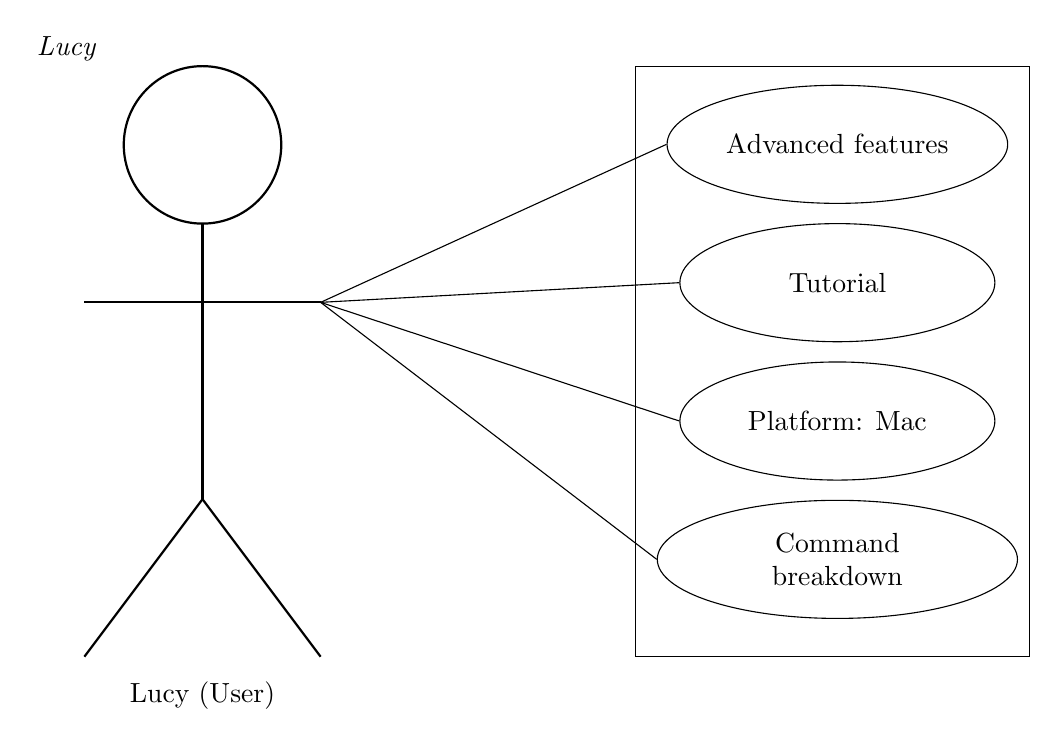
\begin{tikzpicture}[>=latex]
			%elements
			% \draw (0,0) circle (1cm);
			\node [thick] at (0,0) (head) [circle,draw, minimum width=20mm] {};
			\node at ($(head.north west) + (-1cm,0.5cm)$)[] {\itl{Lucy}};
			%torso
			\draw [thick] (canvas cs:x=0cm,y=-10mm) -- (canvas cs:x=0cm,y=-4.5cm);
			%arms
			\draw [thick] (canvas cs:x=-1.5cm,y=-2cm) -- (canvas cs:x=1.5cm,y=-2cm);
			%right leg
			\draw [thick] (canvas cs:x=0cm,y=-4.5cm) -- (canvas cs:x=1.5cm,y=-6.5cm);
			%right leg
			\draw [thick] (canvas cs:x=0cm,y=-4.5cm) -- (canvas cs:x=-1.5cm,y=-6.5cm);
			%name
			\node at (canvas cs:x=0cm,y=-7cm) [] {Lucy (User)};
			%requirements box
			\node at (canvas cs:x=8cm,y=-2.75cm) (box) [rectangle, draw=black!100, minimum width=5cm, minimum height=7.5cm] {};

			% requirements
			\node [right] at ($(box.north west) + (0.4cm, -1cm)$) (req1) [ellipse,draw=black!100,minimum width=4cm,minimum height=1.5cm] {Advanced features};
			\node [] at ($(req1.south) + (0cm, -1cm)$) (req2) [ellipse,draw=black!100,minimum width=4cm,minimum height=1.5cm] {Tutorial};
			\node [] at ($(req2.south) + (0cm, -1cm)$) (req3) [ellipse,draw=black!100,minimum width=4cm,minimum height=1.5cm] {Platform: Mac};
			\node [] at ($(req3.south) + (0cm, -1cm)$) (req4) [ellipse,draw=black!100,minimum width=4cm,minimum height=1.5cm ,text width=3cm, align=center] {Command breakdown};


			\draw [] (req1.west) -- (canvas cs:x=1.5cm,y=-2cm);
			\draw [] (req2.west) -- (canvas cs:x=1.5cm,y=-2cm);
			\draw [] (req3.west) -- (canvas cs:x=1.5cm,y=-2cm);
			\draw [] (req4.west) -- (canvas cs:x=1.5cm,y=-2cm);
		\end{tikzpicture}
    %
    %
  \ssctn{Software Requirement Specification}
  Prototyping is a key component of the Agile methodology, to do so two individual requirement specifications will be developed, one for the prototype and one for the final product. It is important to develop prototypes since they can quickly reveal issues with implementation considerations.
  %
  \sssctn{Prototype}
  The requirements for the prototype form the basis on which the final product will be built.\\\\
  %
  \itl{Functional requirements}\\
  \itm{
    \item Provide the same functionality as the current KoMoDo \itm{
        \item Register banks
				\item Memory view
        \item Breakpoints
        \item Single stepping
        \item Multi stepping
        \item Loading kmd files
        \item Compiling source files
      }
    \item Introduce no additional dependencies\\\\
  }
  %
  \itl{Non-functional requirements}\\
  \itm{
    \item Intuitive design \itm{
        \item Basic view mode
				\item Themes
				\item Action icons
      }
    \item Compatibility: Linux
    \item Similar responsiveness as the current KoMoDo
		\item Create installer for supported platforms\\
  }
  \sssctn{Final Product}
	\itl{Functional requirements}\\
	\itm{
    \item Provide the same functionality as the current KoMoDo \itm{
        \item Register banks \itm{
					\item notify user of register changes
				}
        \item Memory view
        \item Breakpoints
        \item Single stepping
        \item Multi stepping
        \item Loading KMD files
        \item Compiling source files
      }
    \item Introduce no additional dependencies
		\item Syntax highlighting
		\item Breakpoints integrated into memory window
		\item Ability to hide empty memory
		\item More complete build process
		\item Active memory jump-to
		\item Preferences
		\item Themes via XML files
		\item Instruction breakdown\\\\
  }
  %
  \itl{Non-functional requirements}\\
  \itm{
    \item Intuitive design \itm{
        \item Basic view mode
				\item Themes
				\item Action icons
      }
    \item Compatibility: Linux, Windows, Mac
    \item Similar responsiveness as the current KoMoDo
		\item Create installer for supported platforms
  }

%% !TEX root = ./main.tex
\graphicspath{ {images/design/} }
\sctn{Design}
\ssctn{KoMoDo UI breakdown}
\fig{ \centering\img{0.4}{oldkomodo-anno.png} }{Current KoMoDo UI}{currentUI}
KoMoDos current UI leaves alot to be desired.\\\\


\ssctn{Proposed design}
\fig{ \centering\img{0.35}{proposedkomodo.pdf} }{Proposed overhaul}{proposedUI}

%\include{implementation}
%% !TEX root = ./main.tex
\sctn{Testing}
KoMoDo was extensively tested so that first and foremost, no new bugs were introduced and secondly, any pre-existing bugs were removed. Additionally, KoMoDo informally underwent both application and user testing constantly to validate the changes, with only the results of the final round being recorded.
The final round of testing consisted of three stages. System profiling, where KoMoDo was executed using \itl{Valgrind} and \itl{Perf} to detect memory leaks and bottlenecks. Application testing, to determine if the existing and new features all work to a reasonable standard. Finally, user testing, to determine if KoMoDo's changes were valid.\\\\
%
Performance profiling provides developers with information about the runtime of their application. In particular, it was important to profile KoMoDo to ensure that it performs to a high standard on both university and student machines. Of the many profiling methods, two were used, memory checking and performance analysis. Memory checking looks for poor memory management which can introduce memory leaks. Performance analysis looks at the runtime behaviour of the application, providing a breakdown of CPU intensive sections of code.\\\\
%
Application testing was carried out throughout KoMoDo's development, thereby quickly fixing any bugs during the early iterations of development. Any failures are noted in the test-table in the Appendix. Fixes to issues encountered are provided below the original test. Once KoMoDo was complete the tests were executed for a final time to ensure the finished software worked to a high standard. Although the requirements for KoMoDo changed during the development phase, the tests ensured that the new requirements were met.\\\\
%
User testing was informally carried out through the design cycle. By user testing early, KoMoDo's user-interface and user-experience could be better improved. The final round of user testing provides a series of simple tasks which user's need to carry out. The tasks were given to a variety of people.\\\\
%
A suitable test-bench was constructed to carry out the profiling. The test bench and one other system were used for the application testing. System 2 executed KoMoDo inside a virtual machine.\\\\
\bld{\medium{Test-bench}}
\itm{
  \item Intel Next Unit of Computing, model no. NUC5PGYH
  \item 8GB DDR3L 1600MHz
  \item Intel Pentium N3700 2.4GHz quad core
  \item Intel HD Graphics
  \item Operating system: Arch Linux, AMD64, latest stable iteration\\\\
}
%
\bld{\medium{System 2}}
\itm{
  \item Custom PC
  \item Intel i7-6700k 4.00GHz quad core
  \item 32GB DDR4 2400MHz
  \item NVIDEA GTX 1070
  \item Operating system: Windows 10 Pro, AMD16, latest stable iteration
}

\ssctn{Application profiling}
Profiling the memory was done using a piece of software called \itl{Valgrind}. \itl{Valgrind} is a suite which provides various profiling techniques, for KoMoDo, memcheck was used to identify potential memory leaks. \itl{Perf} was used to detail the performance impact of running KoMoDo and identify system bottlenecks. Note, the profiling is done only on KoMoDo and not on the \itl{Jimulator} although, \itl{Perf} will also profile calls to the \itl{Jimulator}. To fairly evaluate KoMoDo's performance a test path was created as shown in Figure \ref{fig: testpath}. The path covers the typical tasks which user's would perform.
%
\fig{
		\centering
		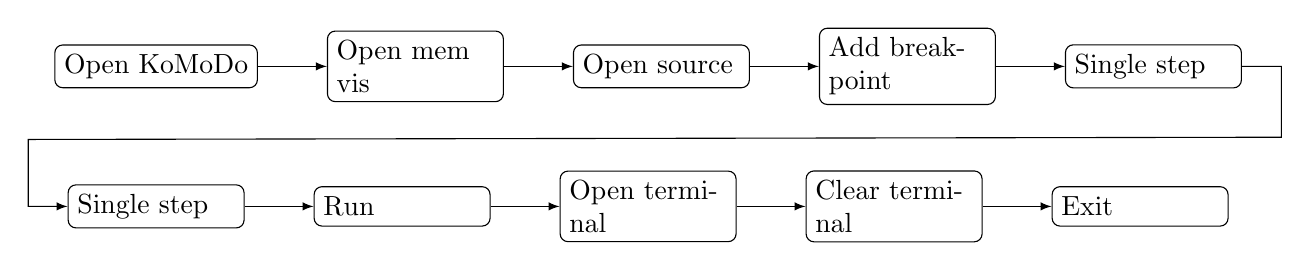
\begin{tikzpicture}[>=latex]
		%elements
		\node [rounded corners=1mm]at (0,0)   (open) [rectangle,draw=black!100, minimum width=20mm, minimum height=5mm] {Open KoMoDo};

		\node [rounded corners=1mm,text width=2cm] at ($(open.east)+(2cm,0cm)$) (largefile) [rectangle,draw=black!100, minimum width=20mm, minimum height=5mm] {Open mem vis};

		\node [rounded corners=1mm,text width=2cm] at ($(largefile.east)+(2cm,0cm)$) (add) [rectangle,draw=black!100, minimum width=20mm, minimum height=5mm] {Open source};

		\node [rounded corners=1mm,text width=2cm] at ($(add.east)+(2cm,0cm)$) (sub) [rectangle,draw=black!100, minimum width=20mm, minimum height=5mm] {Add breakpoint};

		\node [rounded corners=1mm,text width=2cm] at ($(sub.east)+(2cm,0cm)$) (save1) [rectangle,draw=black!100, minimum width=20mm, minimum height=5mm] {Single step};

		\node [rounded corners=1mm,text width=2cm] at ($(open.south)+(0cm,-1.5cm)$) (newfile) [rectangle,draw=black!100, minimum width=20mm, minimum height=5mm] {Single step};

		\node [rounded corners=1mm,text width=2cm] at ($(newfile.east)+(2cm,0cm)$) (options) [rectangle,draw=black!100, minimum width=20mm, minimum height=5mm] {Run};

		\node [rounded corners=1mm,text width=2cm] at ($(options.east)+(2cm,0cm)$) (bg) [rectangle,draw=black!100, minimum width=20mm, minimum height=5mm] {Open terminal};

		\node [rounded corners=1mm,text width=2cm] at ($(bg.east)+(2cm,0cm)$) (line) [rectangle,draw=black!100, minimum width=20mm, minimum height=5mm] {Clear terminal};

		\node [rounded corners=1mm,text width=2cm] at ($(line.east)+(2cm,0cm)$) (write) [rectangle,draw=black!100, minimum width=20mm, minimum height=5mm] {Exit};

		%text
		\draw [->] (open.east) -- (largefile.west);
		\draw [->] (largefile.east) -- (add.west);
		\draw [->] (add.east) -- (sub.west);
		\draw [->] (sub.east) -- (save1.west);
		\draw [->] (save1.east) -- ($(save1.east) + (0.5cm,0cm)$) -- ($(save1.east) + (0.5cm,-0.9cm)$) -- ($(newfile.west) + (-0.5cm,0.85cm)$) -- ($(newfile.west) + (-0.5cm,0cm)$) -- (newfile.west);
		\draw [->] (newfile.east) -- (options.west);
		\draw [->] (options.east) -- (bg.west);
		\draw [->] (bg.east) -- (line.west);
		\draw [->] (line.east) -- (write.west);
		%\draw [->] (write.east) -- ($(write.east) + (0.5cm,0cm)$) -- ($(write.east) + (0.5cm,-0.9cm)$) -- ($(save.west) + (-0.5cm,0.85cm)$) -- ($(save.west) + (-0.5cm,0cm)$) -- (save.west);
		%\draw [->] (save.east) -- (exit.west);
		\end{tikzpicture}
		}{Test path}{testpath}
%
\sssctn{Memory profiling}
Memory profiling identified two instances within KoMoDo which produced memory leaks. One was because an unfreed call \func{g\_strdup} and the other, an unfreed call to \func{g\_strconcat}. Additionally, there were many memory leaks in \itl{GTK1}, which could not be fixed. The leaks in \itl{GTK1} are inline with the rationale behind deprecating some of the original features for being poorly implemented.
\fig{
  \centering
  \begin{varwidth}{\linewidth}
    \verbatiminput{./testing/memleak.txt}
  \end{varwidth}
}{Memory leak originating from unfreed call to \func{g\_strdup}}{memleak}
%
No other leaks were identified within KoMoDo.
%
\sssctn{CPU profiling}
The CPU profiling produced expected results. From Figure \ref{fig: cpuprof} it can be seen that the majority of the cycles are spent on the libraries KoMoDo is built on. KoMoDo overall doesn't have a large resource footprint and any optimizations would be premature and unnecessary.
\fig{
  \centering
  \begin{varwidth}{\linewidth}
    \verbatiminput{./testing/perfcpu-prof.txt}
  \end{varwidth}
}{Usage profile}{cpuprof}

\sssctn{Summary}
In summary, running \itl{Valgrind} provided insight into the poor coding standards of both myself; and the designers of the early \itl{GTK1}. \itl{Perf} confirmed the simplicity of KoMoDo, showing that it is a lightweight ARM32 debugger and emulator.
%
%
%
%
%
\ssctn{Application testing}

%% !TEX root = ./main.tex
\sctn{Reflection}
\ssctn{Problems Encountered}
Problems in software development projects are inevitable. Carefully planning the time required for each task provides a cushion in case of unforeseen circumstances. This cushion allowed me to work around my inexperience with porting software. Additionally, my inexperience required a change to the requirements, however, due to careful planning I had enough time to comfortably complete the required tasks.\\\\
%
The research stage provided me with the opportunity to alleviate some of my inexperience. By researching around KoMoDo my aim was to make an educated decision regarding how best to improve it. However, it is clear to me now that my focus should have been on understanding the intricacies of porting software. The lack of understanding translated poorly to the implementation stage, where, the major problems with porting the legacy software were discovered. I do believe however, that in the future when encountering legacy software I can better identify the potential problems that development will face.\\\\
%
Looking into, and documenting, KoMoDo was no easy task. Countless hours were spent deciphering the cryptic comments or lack there of. I believe that without \itl{GDB}, the GNU Debugger, I would not have understood the convoluted mess that is KoMoDo. From the layout and style of the code it became ever more clear that it was implemented by a single person, over some time. Variables and functions were occasionally in incorrect header files and KoMoDo was rife with comments like; `What does this even do? Magic.'. I do believe however, that thanks to the vague or non-existent comments and \itl{GDB}, I have become better at reading and understanding code. Additionally, I have honed in my skills as a `chameleon' programmer, writing code which mimics the standards of the source. Alternatively, to help future developers better understand KoMoDo, I made sure to comment on the intricate parts of the source, with which I had developed experience.\\\\
%
\itl{GTK1's} documentation has been purged from the internet, this made implementation using \itl{GTK1} very difficult. There exists a small number websites with a subset of the original documentation, these combined with what was already written in KoMoDo allowed me implement new features. Additionally, I used the \itl{GTK2} documentation to supplement what certain functions should do. The process of understanding and using the \itl{GTK1} API was time consuming and laborious, but doing so provided me with the relevant knowledge to carry out the necessary work.\\\\
%
Newer iterations of \itl{GTK} use the UI generation software, \itl{Glade} to design and implement the UI. KoMoDo was built before \itl{Glade's} inception. Consequently, the UI in KoMoDo is hard coded, and uses the \func{.komodo} config file to determine what is drawn to the main view. When attempting to move to \itl{GTK2} it became evident that the UI would need to be developed using \itl{Glade}. On top of \itl{Glade} consistently crashing, the new UI meant that a lot of the existing features in KoMoDo would need to be permanently disabled. They would need to be disabled due to the static structure of the \itl{Glade} files not allowing dynamic UI changes. The loss of features further pushed me into using \itl{GTK1}.
%
%
%
%
\ssctn{Personal Reflection}
I was drawn to this project because of the insight and understanding that the first year module, G51CSA provided me. As a developer the module allowed me to take into consideration the machine level results of my programming decisions. I felt as though KoMoDo needed to be made more accessible to students so that they could also develop this intuition. As one of the key first year modules, in the Computer Science course, at the University of Nottingham, every student is exposed to KoMoDo.\\\\
%
I felt as though my experience until now, as a Computer Science student had best prepared me to take on this challenge. I was both right and wrong, I am able to manage my time efficiently and to quickly implement software requirements. However, my lack of experience with legacy systems and porting software, made this project difficult. I was unable to see the pitfalls of moving from one API to another. Thankfully, due to my time management I was able to work around this oversight and get back on track. I think that I have now gained the relevant experience for future projects.\\\\
%
%how year out helped, experience with modules, c, build tools etc.
I felt as though my year in industry at Intel helped me prepare for this project. Working at Intel exposed me to a variety of technologies and scenarios. Most notably, I worked on a large open source project called MRAA which is on all of Intel's Internet of Things devices. Working on the project exposed me to build tools such as \itl{AutoMake}. Having prior knowledge of using \itl{AutoMake} gave me an advantage when it came to fixing some of the build issues with KoMoDo. Furthermore, working on the open source project allowed me to gain experience looking through someone else's code, understanding what it does and writing useful documentation. All of these skills translated very well when it came to understanding how KoMoDo operated.\\\\
%
At University, I have had the opportunity to build interactive systems, use C and objectively evaluate my choices. All of these opportunities have given me greater insight when working with KoMoDo. Additionally, I was able to make strategic decisions about how best to advance both KoMoDo's UI and, its features so that they adhered to the requirements..\\\\
%
For this particular project I believe that my time management and planning skills really showed. I managed to work around and fix issues that I encountered quickly, producing a high quality piece of work. Using the Agile methodology I setup sprints each week, these sprints were based on the tasks on my Kanban. The flexibility of using sprints allowed me dynamically change my pace so that I could work on other modules when needed. The Kanban allowed me to easily track my progress through the requirements.\\\\
%
%Early and frequent drafts
Although I have already submitted one dissertation, I felt as though my writing skills were still weak. This was further verified during the initial proposal by Professor David Brailsford. My personal aim during this second dissertation was to provide early and often drafts of the write-up. I was lucky that Professor Brailsford was able to consistently provide me with feedback about my work. I believe\footnote{David may disagree} that thanks to his efforts and lectures \footnote{Many grammar lectures} I have improved my technical writing ability.\\\\
%
In summary, I believe that I have thoroughly applied myself doing this dissertation. I have gained valuable expertise in working with legacy systems and their complexity. Furthermore, I believe that I was able to further put into practice the skills I have gained both in industry and via University.
%
%
%
\sssctn{External Reflection}
The original requirements for KoMoDo were not fully met. Lack of experience crippled the implementation stage. However, through my failures, Universities that teach their students using KoMoDo have a better idea of its limitations. Furthermore, thanks to my research and progress a foundation has been established on which KoMoDo can be recreated. Any developer that wishes to develop a modern KoMoDo can refer to my findings and avoid the mistakes I made. I believe that although I did not meet the specification, my work is to a high standard that can be carried on in the future.
%Although the original requirements were not met, the Universities which use KoMoDo now have a better idea about its limitations.
%
%
%
\ssctn{Future Improvements}
I would strongly recommend against any future improvements to KoMoDo as it now exists. Instead KoMoDo should be rebuilt from the ground up. KoMoDo shows signs of the age in which it was created. By using modern frameworks and techniques a `new' KoMoDo would last much longer. Careful planning can make KoMoDo easier to upgrade and maintain in the future.\\\\
%
Any improvements to KoMoDo would be likely to create more problems than solutions. However, there are many ways that KoMoDo can be improved: things such as how code is loaded into the memory or how KMD code is compiled, these can be further refined and streamlined. In the case of code compilation it could be changed to follow a plugin interface, so that users can change the compilation method \itl{ad hoc}. Additionally, rebuilding KoMoDo can allow it to be operating system agnostic, a definite plus for students who may not want to use Linux. KoMoDo was purpose-made to be a generic debugger, able to work with FPGA's, ARM boards and emulators. Although it is no longer used in a production environment, these features should be kept in future iterations.

%\bibliographystyle{plainnat}
%\bibliography{./biblio}
%% !TEX root = ./main.tex
\begin{landscape}
	\newgeometry{left=2cm,bottom=-0.5cm,top=9.1cm}
	\sctn{Testing}
	\ssctn{Application Testing}
  \gdef\rownumber{\stepcounter{magicrownumbers}\arabic{magicrownumbers}}
	\label{apptest}
	\begin{center}
		\begin{tabular}{| @{\makebox[2em][c]{\rownumber\space}} | p{4cm} |  p{5cm} | p{5cm} | p{5cm} | l |}
			\hline
      Input & Precautions & Expected outcome & Actual outcome & Result \\ \hline
			%
			% & & & & & \\ \hline
			%
			Start application & -  & The application starts in emulation mode. & The application starts in emulation mode. & Pass. \\ \hline
			%
			Scroll memory & - & Memory is scrollable and loops back at ranges & Memory is scrollable and loops back at ranges & Pass. \\ \hline
      %
      Switch register banks & - & Register bank can be changed. & Register bank can be changed. & Pass. \\ \hline
      %
      Switch flags & - & Flags easily switched. & Flags easily switched. & Pass.\\ \hline
      %
      Change register value & - &Register value changed. & Register value changed. & Pass.\\ \hline
      %
      Set/unset a flag & - & Flag unset. & Flag unset. & Pass. \\ \hline
      %
      File \rarr Open & Menubar open & Open file dialog. & Open file dialog. & Pass.\\ \hline
      %
      File \rarr Reload & Menubar open & File is reload and compiled if needed. & File is reload and compiled if needed. & Pass. \\ \hline
      %
      Actions \rarr Run & Menubar open & Open sourced is run. & Open sourced is run. & Pass. \\ \hline
      %
      Actions \rarr Pause & Menubar open & Running source is paused. & Running source is paused. & Pass. \\ \hline
      %
      Actions \rarr Stop & Menubar open & Running source is stopped and reset. & Running source is stopped and reset. & Pass. \\ \hline
      %
      Actions \rarr Ping & Menubar open & Board pinged. & Board pinged. & Pass. \\ \hline
      %
      Actions \rarr Single-step & Menubar open & Code is stepped by 1. & Code is stepped by 1. & Pass. \\ \hline
      %
      Actions \rarr Multi-step \rarr steps in input & Menubar open & Code is stepped as in input box. & Code is stepped as in input box. & Pass. \\ \hline
      %
      Actions \rarr Multi-step \rarr 10 steps& Menubar open & Code stepped by 10. & Code stepped by 10. & Pass.\\ \hline
      %
      Actions \rarr Multi-step \rarr 100 steps & Menubar open & Code stepped by 100. & Code stepped by 100. & Pass. \\ \hline
      %
      Actions \rarr Multi-step \rarr 1000 steps & Menubar open & Code stepped by 1000. & Code stepped by 1000. & Pass. \\ \hline
      %
      Actions \rarr Multi-step \rarr 10,000 steps & Menubar open & Code stepped by 10,000. & Code stepped by 10,000. & Pass. \\ \hline
      %
      Actions \rarr Multi-step \rarr 100,000 steps & Menubar open & Code stepped by 100,000. & Code stepped by 100,000. & Pass. \\ \hline
      %
      Actions \rarr Multi-step \rarr 1,000,000 steps & Menubar open & Code stepped by 1,000,000. & Code stepped by 1,000,000. & Pass.\\ \hline
      %
    	\end{tabular}
	\end{center}
%
\begin{center}
  \begin{tabular}{ | @{\makebox[2em][c]{\rownumber\space}} | p{4cm} |  p{5cm} | p{5cm} | p{5cm} | l |}
    \hline
    Input & Precautions & Expected outcome & Actual outcome & Result \\ \hline
    %
    Actions \rarr walk \rarr Steps in input & Menubar open & Source is stepped based on input. & Output is stepped based on input. & Pass. \\ \hline
    %
    Actions \rarr walk \rarr 1 step at a time & Menubar open & Source is stepped one at a time. & Source is stepped one at a time. & Pass. \\ \hline
    %
    Actions \rarr walk \rarr 10 step at a time & Menubar open & Source is stepped 10 at a time. & Source is stepped 10 at a time. & Pass. \\ \hline
    %
    Actions \rarr walk \rarr 100 step at a time & Menubar open & Source is stepped 100 at a time. & Source is stepped 100 at a time. & Pass. \\ \hline
    %
    Actions \rarr walk \rarr 1000 step at a time & Menubar open & Source is stepped 1000 at a time. & Source is stepped 1000 at a time. & Pass. \\ \hline
    %
    Actions \rarr toggle refresh & Menubar open & Refresh is toggled. & Refresh is toggled. & Pass. \\ \hline
    %
    Special \rarr Breakpoints & Menubar open & Show advanced breakpoint window. & Shown advanced breakpoint window. & Pass. \\ \hline
    %
    Special \rarr Simple Breakpoints & Menubar open & Show simple breakpoint window. & Shown simple breakpoint window. & Pass. \\ \hline
    %
    Special \rarr Watchpoints & Menubar open & Show advanced watchpoint window. & Shown advanced watchpoint window. & Pass. \\ \hline
    %
    Special \rarr Simple Watchpoints & Menubar open & Show simple watchpoint window.  & Shown simple watchpoint window. & Pass. \\ \hline
    %
    Special \rarr Memory Window & Menubar open & Show memory window. & Shown memory window. & Pass. \\ \hline
    %
    Special \rarr Source window & Menubar open & Show source window & Shown source window. & Pass. \\ \hline
    %
    Special \rarr Symbol window & Menubar open & Show symbol window & Shown Symbol window & Pass. \\ \hline
    %
    Special \rarr Mem vis & Menubar open & Show mem vis & Shown mem vis & Pass. \\ \hline
    %
    Special \rarr Features & Menubar open & Show Features window & Shown Features window & Pass. \\ \hline
    %
    Reg. Bank \rarr any option & Menubar open & Switch Reg. bank & Switched current Reg. bank & Pass. \\ \hline
    %
    Flags \rarr any option & Menubar open & Switches flags & Switches flags & Pass. \\ \hline
    %
    Help \rarr about & Menubar open & Opens about window & Opens about window & Pass. \\ \hline
    %
    Open Button & - & Open file dialog & Open file dialog & Pass. \\ \hline
    %
    Reload button & - & Opened source is reloaded & Opened source is reloaded & Pass. \\ \hline
    %
    Features button & - & Show features window & Shown features window & Pass. \\ \hline
    %
    Play button & - & Run source & Runs source & Pass. \\ \hline
    %
    Pause button & - & Pauses execution of source & Pauses execution of source & Pass. \\ \hline
    %
    Stop button & - & Stops and resets execution of source & Stops and resets execution of source & Pass. \\ \hline
    %
    Refresh button & - & Button is toggled & Button is toggled & Pass. \\ \hline
    %
    \end{tabular}
\end{center}
%
\begin{center}
  \begin{tabular}{ | @{\makebox[2em][c]{\rownumber\space}} | p{4cm} |  p{5cm} | p{5cm} | p{5cm} | l |}
    \hline
    Input & Precautions & Expected outcome & Actual outcome & Result \\ \hline
  Single-step button & - & Source is single stepped & Source is single stepped & Pass. \\ \hline
  %
  Multi-step button & - & Source is stepped based on input box & Source is stepped based on input box & Pass. \\ \hline
  %
  Timed walk button & - & Source is walked based on input box & Source is walked based on input box & Pass. \\ \hline
  %
  Multi-step input & - & Value can be manually changed & Value can be manually changed & Pass. \\ \hline
  %
  Multi-step input & - & Value can be changed using buttons & value changed using buttons & Pass. \\ \hline
  %
  Timed walk input & - & Value can be manually changed & Value can be manually changed & Pass. \\ \hline
  %
  Timed walk input & - & Value can be changed using buttons & Value can be changed using buttons & Pass. \\ \hline
  %
  Breakpoint checkbox & - & Activates/deactivates Breakpoints & Activates/deactivates Breakpoints & Pass. \\ \hline
  %
  Watchpoint checkbox & - & Activates/deactivates Watchpoints & Activates/deactivates Watchpoints & Pass. \\ \hline
  %
  SWI checkbox & - & Enters software interrupt & Enters software interrupt & Pass. \\ \hline
  %
  BL checkbox & - & Enters sub-routine & Enters sub-routine & Pass. \\ \hline
  %
  Abort checkbox & - & Enters bad memory exception code & Enters bad memory exception code & Pass. \\ \hline
  %
  IRQ checkbox & - & Automatically executes interrupt & Automatically executes interrupt & Pass. \\ \hline
  %
  FIQ checkbox & - & Automatically executes FIQ code & Automatically executes FIQ code & Pass. \\ \hline
  %
  Memory window single step & - & Single steps the code & Single steps the code & Pass. \\ \hline
  %
  Address jump input & - & Jumps to memory address & Jumps to memory address & Pass. \\ \hline
  %
  Full source checkbox & - & Toggles between full and partial source & Toggles between full and partial source & Pass. \\ \hline
  %
  Symbols checkbox & - & Toggles between showing/not showing symbols & Toggles between showing/not showing symbols & Pass. \\ \hline
  %
  Status bar: Mode & KoMoDo started using -e flag & Shows KoMoDo in emulation mode & Shows KoMoDo in emulation mode & Pass. \\ \hline
  %
  Status bar: State & Any actions involving the code & State changes when program controls are used & State changes when program controls are used & Pass. \\ \hline
  %
  Status bar: Total steps & during execution & Shows \# of steps taken & Shows \# of steps taken & Pass. \\ \hline
  %
  Status bar: Load Progress & After open dialog & Shows progress status when loading source & Shows progress status when loading source & Pass. \\ \hline
  %
  \end{tabular}
  \end{center}
  \begin{center}
  \begin{tabular}{ | @{\makebox[2em][c]{\rownumber\space}} | p{4cm} |  p{5cm} | p{5cm} | p{5cm} | l |}
      \hline
      Input & Precautions & Expected outcome & Actual outcome & Result \\ \hline
      %
      KoMoDo console window & During source loading & Shows output from compilation and any errors & Shows output from compilation and any errors & Pass. \\ \hline
      %
      Memory window: tabs & - & Increases the size of the tabs in the memory window & Increases the size of the tabs in the memory window & Pass. \\ \hline
      %
      Memory window: Up button & - & Scrolls up & Scrolls up & Pass. \\ \hline
      %
      Memory window: Down button & - & Scrolls down & Scrolls down & Pass. \\ \hline
      %
      Memory window: Add breakpoint & line does not already have breakpoint & Breakpoint added & Breakpoint added & Pass.\\ \hline
      %
      Memory window: Remove breakpoint & Line has breakpoint & Breakpoint removed & Breakpoint removed & Pass.\\ \hline
      %
      Memory window: Slider & - & Moves memory when moved up or down & Moves memory when moved up or down & Pass.\\ \hline
      %
      Memory window: Scroll & - & Moves memory window & Moves memory window & Pass.\\ \hline
      %
      Terminal: running source & Features pressed in emulation mode & SWI3's print to terminal & SWI3's print to terminal & \\ \hline
      %
      Terminal: clear button & Features pressed in emulation mode & Button clears view & Button clears view & Pass.\\ \hline
      %
      Terminal: Active checkbox & Features pressed in emulation mode & toggles printing output to terminal & toggles printing output to terminal & Pass.\\ \hline
      %
      Memvis: close & Memvis open & Closes memory visualisation & Closes memory visualisation & Pass.\\ \hline
      %
      Memvis: memory visual & Memvis open & Shows taken sectors & Shows taken sectors & Pass.\\ \hline
      %
      Symbol table & Symbol table open & Shows list of symbols & Shows list of symbols & Pass.\\ \hline
      %
      File compiled and loaded & Open file dialog & File is compiled and loaded after it is selected &File is compiled and loaded after it is selected & Pass. \\ \hline
      %
      Unknown file & Open file dialog & Unknown format not compiled or loaded showing dialog box & Unknown format not compiled or loaded showing dialog box & Fail. \\ \hline
      %
      Unknown file & Open file dialog & Unknown format not compiled or loaded showing dialog box & Unknown format not compiled or loaded showing dialog box & Pass. \\ \hline
      %
      & & & & \\ \hline
      %
      & & & & \\ \hline
      %
  \end{tabular}
  \end{center}
  \restoregeometry
	\end{landscape}


\end{document}
